% Created 2020-09-11 Fri 09:24
% Intended LaTeX compiler: pdflatex
\documentclass[aspectratio=169,presentation]{beamer}
\usepackage[utf8]{inputenc}
\usepackage[T1]{fontenc}
\usepackage{graphicx}
\usepackage{grffile}
\usepackage{longtable}
\usepackage{wrapfig}
\usepackage{rotating}
\usepackage[normalem]{ulem}
\usepackage{amsmath}
\usepackage{textcomp}
\usepackage{amssymb}
\usepackage{capt-of}
\usepackage{hyperref}
\usepackage{tikz}
\usepackage[newfloat]{minted}
\usepackage[spanish]{babel}
\usepackage{tikz}
\usepackage{minted}
\setmonofont{Iconsolata}
\usetheme{Madrid}
\author{Gustavo Puche}
\date{\today}
\title{Introducción al c++ moderno}
\hypersetup{
 pdfauthor={Gustavo Puche},
 pdftitle={Introducción al c++ moderno},
 pdfkeywords={},
 pdfsubject={},
 pdfcreator={Emacs 27.0.50 (Org mode 9.3.8)}, 
 pdflang={Spanish}}
\begin{document}

\maketitle
\begin{frame}{Outline}
\tableofcontents
\end{frame}

\section{Introducción}
\label{sec:orgd3c494d}
\begin{frame}[label={sec:org89aa207}]{Introducción}
\begin{itemize}
\item Objetivos
\item Motivación
\item Bases del lenguaje
\item Definición de tipos
\item Modularidad
\item Gestión de memoria
\item Clases
\item Operaciones esenciales
\item Librería estándar
\item Uso de lambdas
\item Programación genérica (templates)
\item Conclusiones
\end{itemize}
\end{frame}
\begin{frame}[label={sec:org4612eaa}]{Objetivos}
Dar las bases para la programación moderna en C++11 y superiores.
\end{frame}
\begin{frame}[label={sec:orge2f4ecd}]{Motivación}
\begin{itemize}
\item Gran demanda de proyectos en esta tecnología
\item Lenguaje de alto rendimiento
\item Lenguaje moderno y actualizado
\item Programación funcional
\item Programación genérica
\end{itemize}
\end{frame}
\section{Bases del Lenguaje}
\label{sec:org20d2171}
\begin{frame}[label={sec:org20faec7}]{Bases del Lenguaje}
\begin{itemize}
\item Tipos básico
\item Sentencias
\end{itemize}
\end{frame}
\begin{frame}[label={sec:orgd5c0b9c}]{Tipos básicos}
\begin{itemize}
\item Tipos Básico
\item Punteros
\item Referencias
\item cons
\item consexpr
\end{itemize}
\end{frame}
\begin{frame}[label={sec:orgf5cf01c},fragile]{Tipos básicos}
 \begin{minted}[breaklines,fontsize=\small,tabsize=2,frame=lines,autogobble]{c++}
bool   // Boolean. Valores posibles true y false
char   // Carácter. Ejemplos: 'a', 'z', y '9'
int    // Entero. Ejemplos: -273, 42, y 1066
double // Número decimal. Ejemplos:-273.15, 3.14, y 6.626e-34
       // Enteros positivos. Ejemplos: 0, 1, y 999
\end{minted}
\begin{block}{Tamaño de los tipos en bytes}
\begin{center}
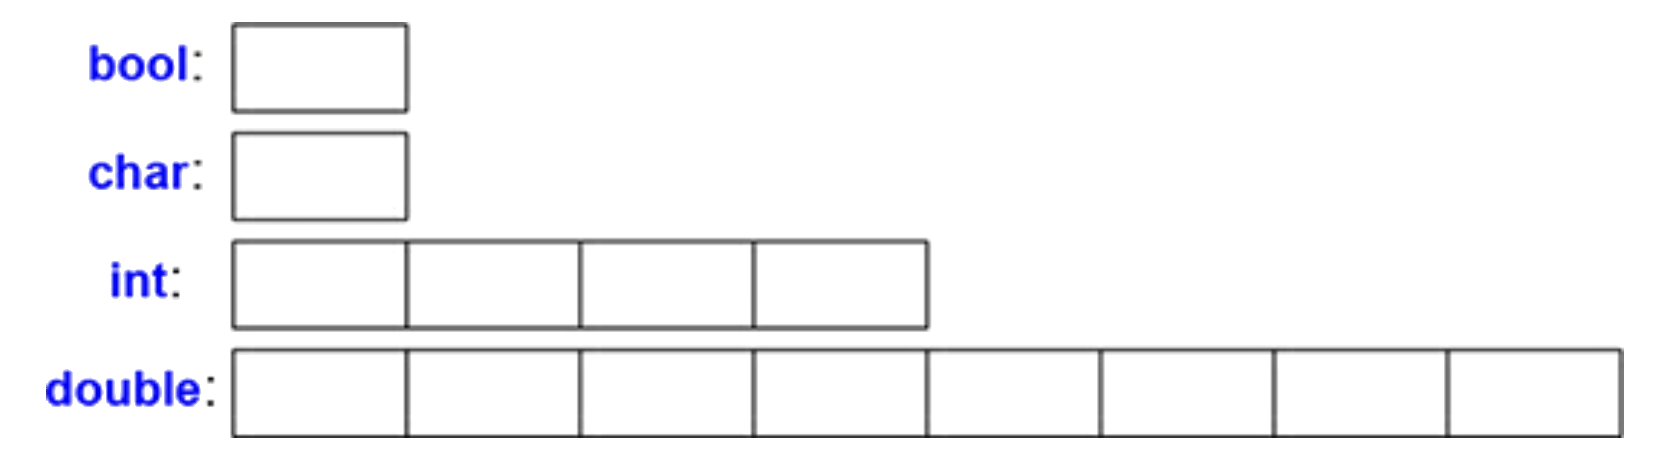
\includegraphics[width=.9\linewidth]{./img/type-size.png}
\end{center}
\end{block}
\end{frame}
\begin{frame}[label={sec:org78e0362}]{Tipos básicos}
\begin{itemize}
\item Arrays, punteros y referencias
\end{itemize}
\begin{center}
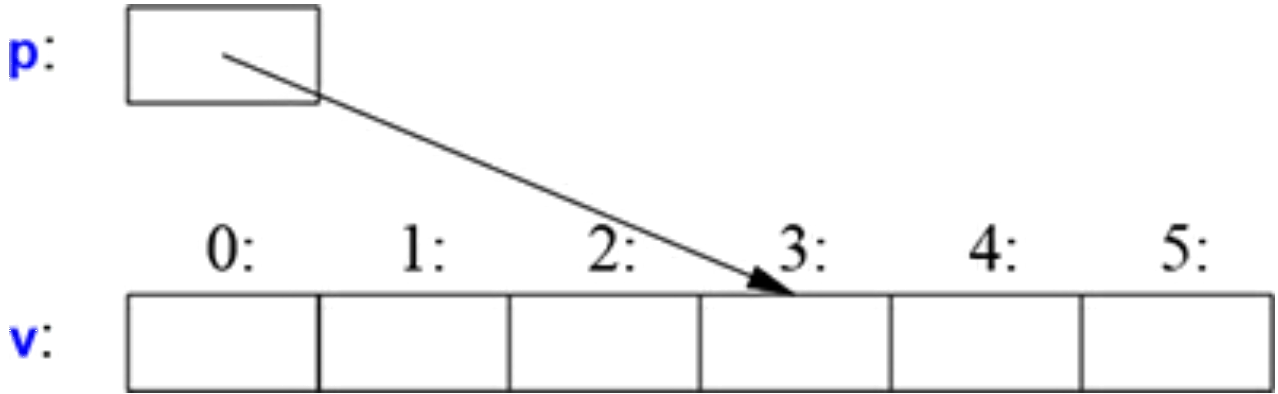
\includegraphics[width=.9\linewidth]{./img/pointer-paint.png}
\end{center}
\end{frame}
\begin{frame}[label={sec:org4fa94ff},fragile]{Tipos básicos}
 \begin{itemize}
\item Punteros
\item Referencias
\end{itemize}
\begin{minted}[breaklines,fontsize=\small,tabsize=2,frame=lines,autogobble]{c++}
int num = 3;
int p1* = &num;

int v[10] = {0,1,2,3,4,5,6,7,8,9};

int p* = &v[3];
\end{minted}
\end{frame}
\begin{frame}[label={sec:org3db2406},fragile]{Tipos básicos}
 Las constantes en \texttt{C++} son de 2 tipos:
\begin{columns}
\begin{column}{0.48\columnwidth}
\begin{block}{\texttt{const}}
\begin{itemize}
\item Prohíbe que se modifique una variables.
\item Es usado generalmente en la definición de interfaces
\item Puede ser calculado en tiempo de ejecución.
\end{itemize}
\end{block}
\end{column}
\begin{column}{0.48\columnwidth}
\begin{block}{\texttt{constexpr}}
\begin{itemize}
\item Calculado en tiempo de compilación.
\item El compilador evalúa la expresión y la sustituye por su valor.
\end{itemize}
\end{block}
\end{column}
\end{columns}
\end{frame}
\begin{frame}[label={sec:org2e47262},fragile]{cons y consexpr}
 \begin{minted}[breaklines,fontsize=\small,tabsize=2,frame=lines,autogobble]{c++}
constexpr double square(double x) { return x*x;}
double sum(const vector<double>&); // sum no puede modificar su argumento.

vector<double> v{1.2,3.4,4.5}; // v no es una constante.

const double s1 = sum(v); // Correcto.
constexpr double s2 = sum(v) // Error: sum(v) no es una expresión constante.

\end{minted}
\end{frame}
\begin{frame}[label={sec:org48583da}]{Sentencias}
\begin{itemize}
\item Bloques
\begin{itemize}
\item if
\item switch
\end{itemize}
\item Bucles
\begin{itemize}
\item while
\item for
\end{itemize}
\end{itemize}
\end{frame}
\begin{frame}[label={sec:org347b919},fragile]{Ejemplo de bloque de código}
 \begin{minted}[breaklines,fontsize=\small,tabsize=2,frame=lines,autogobble]{c++}
void BubbleSort(int *A, int n, bool (*fptr)(int,int))
{
	int i,j,temp;
	for (i = 0; i < n; i++)
		for (j = 0; j < n - 1; j++)
		{
			if (fptr(A[j],A[j+1])) // true if SWAP is needed.
			{
				temp = A[j];
				A[j] = A[j+1];
				A[j+1]= temp;
			}
		}
}
\end{minted}
\end{frame}
\section{Definición de tipos}
\label{sec:orgae5f848}
\begin{frame}[label={sec:org790b76a}]{Definición de tipos}
\begin{itemize}
\item Estructuras
\item Clases
\item Uniones
\item Enumeraciones
\end{itemize}
\end{frame}

\begin{frame}[label={sec:org35f42d3}]{Definición de tipos}
\begin{columns}
\begin{column}{0.48\columnwidth}
\begin{block}{Estructuras}
\begin{itemize}
\item Las estructuras mantienen separados los datos de las operaciones.

\item Por defecto los miembros de una estructura son de acceso público.
\end{itemize}
\end{block}
\end{column}
\begin{column}{0.48\columnwidth}
\begin{block}{Clases}
\begin{itemize}
\item Las clases agrupan los datos y las operaciones sobre estos.

\item Esto permite proteger los datos y las operaciones de los usuarios.

\item Por defecto los miembros de una clase son de acceso privado.
\end{itemize}
\end{block}
\end{column}
\end{columns}
\end{frame}
\begin{frame}[label={sec:org6465500},fragile]{Estructuras}
 \begin{minted}[breaklines,fontsize=\small,tabsize=2,frame=lines,autogobble]{c++}
struct Image
{
	int     nrows, ncols; // Number of rows and columns.
	int**   pixels;       // Pointer to image pixels.
};
\end{minted}
\end{frame}

\begin{frame}[label={sec:orga9cfb8d},fragile]{Clases}
 \begin{minted}[breaklines,fontsize=\small,tabsize=2,frame=lines,autogobble]{c++}
class Image
{
 public:
  Image();
  Image(int n, int m, int g); // Fills pixels n x m with g value
  Image(const Image& I);      // Copy Constructor
  ~Image() ;                  // Destructor

  const Image& operator= (const Image&); // Assign operator

  int  getNrows();  // Rows
  int  getNcols();  // Columns
  int  getGray(int x, int y) const;  // Gray pixel value (x,y).
  void setGray(int x, int y, int g); // Set pixel value (x,y).

	[...]
};
\end{minted}
\end{frame}
\begin{frame}[label={sec:org8ad4073},fragile]{Clases}
 \begin{minted}[breaklines,fontsize=\small,tabsize=2,frame=lines,autogobble]{c++}
class Image
{
  [...]

 private:
  int nrows, ncols; // Number of rows and columns.
  int **pixels;     // Pointer to image pixels.

  void reserveMemory();       // Reserves memory.
  void copy (const Image& I); // Copy I image over current image.
  void freeMemory();          // Frees memory.
};
\end{minted}
\end{frame}
\begin{frame}[label={sec:orge188c51},fragile]{Uniones}
 \begin{block}{Unión}
Es una estructura en la que sus elementos ocupan la misma posición de memoria.

Solo se puede escoger uno de los elementos a la vez.
\note{variant
La solución a los errores derivado del colapso de direcciones de
memoria de los elementos es mejor usar \texttt{variant}.}
\end{block}
\end{frame}
\begin{frame}[label={sec:org8d77246},fragile]{Uniones}
 \begin{minted}[breaklines,fontsize=\small,tabsize=2,frame=lines,autogobble]{c++}
union Pixel
{
	RGB p;
	int gray;
};
struct Image
{
	int       nrows, ncols; // Number of rows and columns.
	Pixel**   pixels;       // Pointer to image pixels.
	Image();
};
[...]
Image im;
im.pixels[5][5].p.r = 180;
im.pixels[5][5].p.g = 50;
im.pixels[5][5].p.b = 190;
	
im.pixels[5][6].gray = 250;
\end{minted}
\end{frame}
\begin{frame}[label={sec:org625c113},fragile]{Enumeraciones}
 \begin{block}{Enum}
Permite definir un conjunto de valores que enumeran una cualidad.

Por ejemplo podemos definir color como rojo, verde y azul.
\end{block}
\begin{block}{}
\begin{minted}[breaklines,fontsize=\small,tabsize=2,frame=lines,autogobble]{c++}
enum color {rojo,verde, azul};
\end{minted}
\note{Colisión de nombres
Ejemplo que muestra que ocurre cuando el nombre de un elemento está
presente en 2 enumeraciones.

Solución: enumName::enumElem.}
\end{block}
\end{frame}
\begin{frame}[label={sec:orgdb26007},fragile]{Enumeraciones}
 \begin{minted}[breaklines,fontsize=\small,tabsize=2,frame=lines,autogobble]{c++}
enum ImageType {grayscale, color};
[...]
int main()
{
	Image im{color};

	if (im.type == color)
	{
		im.pixels[5][5].p.r = 180;
		im.pixels[5][5].p.g = 50;
		im.pixels[5][5].p.b = 190;
	}
	else
	{
		im.pixels[5][5].gray = 250;
	}
}
\end{minted}
\end{frame}

\section{Modularidad}
\label{sec:org3ce2ff1}
\begin{frame}[label={sec:org47a6bc9}]{Modularidad}
\begin{columns}
\begin{column}{0.48\columnwidth}
\begin{block}{Programa C++}
Formado por diferentes partes separadas entre sí.
\begin{itemize}
\item Interfaz
\item Implementación
\end{itemize}
\end{block}
\end{column}
\end{columns}
\end{frame}
\begin{frame}[label={sec:orge4d29e2},fragile]{Modularidad}
 \begin{block}{Interfaces}
Se suelen definir en los archivos de cabecera con extensión \texttt{.h}

Representan las declaraciones que contienen todo lo
necesario para usar una función o tipo.
\end{block}
\end{frame}

\begin{frame}[label={sec:orge0ec134},fragile]{}
 \begin{minted}[breaklines,fontsize=\small,tabsize=2,frame=lines,autogobble]{c++}
class Image
{
	int nrows, ncols; // Number of rows and columns.
  int **pixels;     // Pointer to image pixels.

  void reserveMemory();       // Reserves memory.
  void copy (const Image& I); // Copy I image over current image.
  void freeMemory();          // Frees memory.

 public:
  Image();
  Image(int n, int m, int g); // Fills pixels n x m with g value
  Image(const Image& I);      // Copy Constructor
  ~Image();                   // Destructor

  const Image& operator= (const Image&); // Assign operator

  int  getNrows();  // Rows
  int  getNcols();  // Columns
  int  getGray(int x, int y) const;  // Gray pixel value (x,y).
  void setGray(int x, int y, int g); // Set pixel value (x,y).

	Image operator+ (const Image& I); //Add Images
  Image operator- (const Image& I); //Sub Images
  Image operator! ();   // Invierte la Image
};
\end{minted}
\end{frame}
\begin{frame}[label={sec:orge977b4a},fragile]{Modularidad}
 \begin{block}{Implementación}
Se definen en uno o varios ficheros con extensión \texttt{.cpp}

Representan las definiciones de los tipos o funciones.
\end{block}
\end{frame}

\begin{frame}[label={sec:org6bd25ae},fragile]{Implementación}
 \begin{minted}[breaklines,fontsize=\small,tabsize=2,frame=lines,autogobble]{c++}
#include<imageInterface.h>
using namespace std;
	
Image::Image(int rows, int cols, int g)
{
	nrows = rows;
	ncols = cols;
	
	pixels = new int*[rows];
	for (int i = 0; i < rows; i++)
	{
		pixels[i] = new int[cols];

		for (int j = 0; j < cols; j++)
		{
			pixels[i][j] = g;
		}
	}
}
\end{minted}
\end{frame}
\begin{frame}[label={sec:orgac5be71}]{Modularidad}
\begin{block}{Compilación separada}
\begin{itemize}
\item Los fichero .cpp se compilan por separado generando fichero objeto
(.o o .obj).
\item Esta compilación separada permite modificar una clase sin necesidad
de recompilar el programa entero.
\end{itemize}
\end{block}
\end{frame}
\begin{frame}[label={sec:org5dbb545},fragile]{Compilación separada}
 \begin{minted}[breaklines,fontsize=\small,tabsize=2,frame=lines,autogobble]{c++}
// imageModule.cpp

#include<imageInterface.h>

using namespace std;

int main()
{
  Image im{10,10,200};
    
  cout << "imageImplementation is finnished." << endl;
}
\end{minted}
\end{frame}
\begin{frame}[label={sec:org603e67e}]{Compilación separada}
\begin{alertblock}{¡Atención!}
\begin{itemize}
\item Un cambio en un fichero de implementación .cpp implicará recompilar
el fichero y realizar el enlazado.
\item Un cambio en un fichero de interfaz .h implicará recompilar todos
los ficheros .cpp que la incluyen.
\end{itemize}
\note{variant
\begin{itemize}
\item Preparar una imagen con unos ladrillos que representan el código
objeto resultado del compilador y la argamasa que es la unión de los
diferentes bloques que realiza el enlazador (linker).
\item La imagen de base ya está en la carpeta img.
\end{itemize}}
\end{alertblock}
\end{frame}
\begin{frame}[label={sec:orgd04131f}]{Modularidad}
\begin{columns}
\begin{column}{0.28\columnwidth}
\begin{block}{Namespaces}
\begin{itemize}
\item Ofrecen un nivel superior de organización al de las clases y las
enumeraciones.
\item Permiten evitar conflictos de nombres.
\end{itemize}
\end{block}
\end{column}
\begin{column}{0.48\columnwidth}
\begin{center}
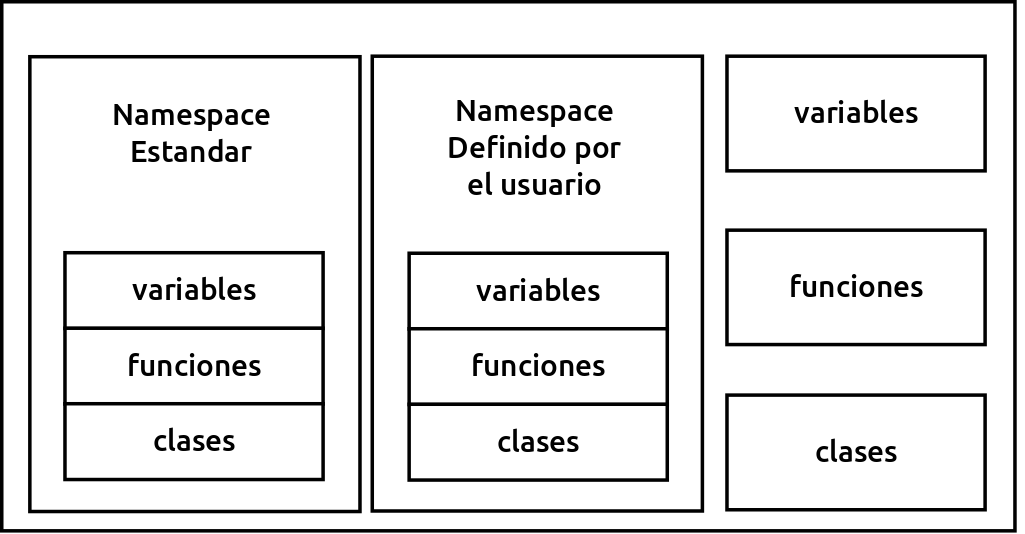
\includegraphics[width=.9\linewidth]{./img/namespaces.png}
\end{center}
\end{column}
\end{columns}
\end{frame}

\begin{frame}[label={sec:org313389b},fragile]{Namespaces}
 \begin{minted}[breaklines,fontsize=\small,tabsize=2,frame=lines,autogobble]{c++}
namespace gray
{
	class Image
	{
		int nrows, ncols; // Number of rows and columns.
		int **pixels;     // Pointer to image pixels.
		
		void reserveMemory();       // Reserves memory.
		void copy (const Image& I); // Copy I image over current image.
		void freeMemory();          // Frees memory.
		
	public:
		Image();
		Image(int n, int m, int g); // Fills pixels n x m with g value
}
\end{minted}
\end{frame}
\begin{frame}[label={sec:orge070dc8},fragile]{Namespaces}
 \begin{minted}[breaklines,fontsize=\small,tabsize=2,frame=lines,autogobble]{c++}
namespace rgb
{
	struct RGB
	{
		int r,g,b;
	};
		
	class Image
	{
		int nrows, ncols; // Number of rows and columns.
		RGB **pixels;     // Pointer to image pixels.
		
		void reserveMemory();       // Reserves memory.
		void copy (const Image& I); // Copy I image over current image.
		void freeMemory();          // Frees memory.
		
	public:
		Image();
		Image(int n, int m, int r, int g, int b); // Fills pixels n x m with rgb value
}
\end{minted}
\end{frame}
\begin{frame}[label={sec:org84f26fd},fragile]{Namespaces}
 \begin{minted}[breaklines,fontsize=\small,tabsize=2,frame=lines,autogobble]{c++}
gray::Image::Image(int rows, int cols, int g)
{
 [...]
}
rgb::Image::Image(int rows, int cols, int r, int g, int b)
{
 [...]
}
\end{minted}
\end{frame}

\section{Gestión de memoria}
\label{sec:org24be6cc}
\begin{frame}[label={sec:orgbb76bd9}]{Gestión de memoria}
\begin{columns}
\begin{column}{0.48\columnwidth}
\begin{itemize}
\item C++ hereda de C un control fino de la memoria dinámica usada por el programa.
\item El sistema operativo divide la memoria de programa en bloques.
\end{itemize}
\end{column}
\begin{column}{0.28\columnwidth}
\begin{center}
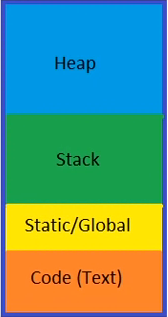
\includegraphics[width=.9\linewidth]{./img/heap-stack-color.png}
\end{center}
\end{column}
\end{columns}
\end{frame}
\begin{frame}[label={sec:org711ae77},fragile]{Gestión de memoria}
 \begin{columns}
\begin{column}{0.48\columnwidth}
\begin{block}{Memoria de programa}
\begin{itemize}
\item Code (Text): Área para el código máquina del programa.
\item Static/Global: Área para las variables globales del programa.
\item Stack: Área para las variables locales y la pila de programa.
\begin{itemize}
\item El tamaño de esta área es fijo, si se supera se produce el error
\end{itemize}
\texttt{Stack Overflow}.
\item Heap (Free Store): Área de memoria dinámica.
\begin{itemize}
\item El tamaño de esta área es virtualmente la memoria del equipo.
\end{itemize}
\end{itemize}
\end{block}
\end{column}
\begin{column}{0.28\columnwidth}
\begin{center}
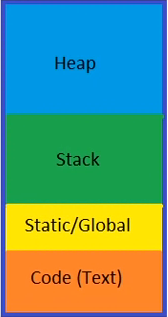
\includegraphics[width=.9\linewidth]{./img/heap-stack-color.png}
\end{center}
\end{column}
\end{columns}
\end{frame}
\begin{frame}[label={sec:org950a301}]{Gestión de memoria dinámica}
\begin{columns}
\begin{column}{0.48\columnwidth}
\begin{block}{Herencia de C}
\begin{itemize}
\item malloc
\item free
\item calloc
\item realloc
\end{itemize}
\end{block}
\end{column}
\begin{column}{0.48\columnwidth}
\begin{block}{C++}
\begin{itemize}
\item new
\item delete
\end{itemize}
\end{block}
\end{column}
\end{columns}
\end{frame}
\begin{frame}[label={sec:orgc171c7e},fragile]{Gestión de memoria dinámica}
 \begin{minted}[breaklines,fontsize=\small,tabsize=2,frame=lines,autogobble]{c++}
Pixel**   pixels;       // Pointer to image pixels.

pixels = new Pixel*[rows];
for (int i=0;i<10;i++)
{
	pixels[i] = new Pixel[cols];
}		

int * copy;

copy = (int*)malloc(im.nrows*im.ncols*sizeof(int));
\end{minted}
\end{frame}
\section{Clases}
\label{sec:org2c3c6cc}
\begin{frame}[label={sec:org819730a}]{Clases}
\begin{block}{Definición}
Tipo definido por el usario para representar un concepto.
\end{block}
\begin{block}{Principales cualidades}
\begin{itemize}
\item Agrupan los datos y las operaciones sobre estos.
\item Proteger los datos y las operaciones de usuarios maintencionados.
\begin{itemize}
\item Por defecto, sus miembros son de acceso privado.
\end{itemize}
\item Permiten sobrecargar las operaciones para diferente dato de entrada.
\item Permiten derivar typos más complejos que heredan sus características básicas.
\end{itemize}
\end{block}
\end{frame}
\begin{frame}[label={sec:org1f23314}]{Clases}
\begin{block}{Tipos de clases}
\begin{itemize}
\item Clases concretas
\item Clases abstractas
\item Clases en las jerarquía de clases
\end{itemize}
\end{block}
\end{frame}
\begin{frame}[label={sec:org9b62f40}]{Clases concretas (Tipos concretos)}
\begin{itemize}
\item En C++ todo son clases por ser un lenguaje orientado a objetos.
\item Las clases concretas son similires a los tipos básicos suministrados por las librerías básicas de C++.
\item Su representación es parte de su definición, lo que permite que las implementaciones sean eficientes en tiempo y espacio.
\end{itemize}
\begin{block}{Características}
\begin{itemize}
\item Instancia sus datos en la memoria estática (stack).
\item No usa punteros.
\item Inicializa automáticamente los objetos.
\item Copia y muebe objetos.
\end{itemize}
\end{block}
\end{frame}
\begin{frame}[label={sec:org2ae5f3c},fragile]{}
 \begin{minted}[breaklines,fontsize=\small,tabsize=2,frame=lines,autogobble]{c++}
// pixel.h
#include<stdio.h>
#include <iostream>

using namespace std;

namespace rgb
{
	class Pixel
	{
		int r,g,b; // Pixel components.
	public:		
		Pixel(){
			r = g = b = 0;
		}
		
		Pixel(int r, int g, int b){ // Fills pixel with rgb value.
			this->r = r;
			this->g = g;
			this->b = b;
		}
				
		Pixel operator+(const Pixel& p){ // Add 2 Pixels.
			Pixel res;
			res.r = r + p.r; // Add pixel components
			res.g = g + p.g;
			res.b = b + p.b;
			return res; // and return the result.
		}

		int getR() const { return r;}
		int getG() const { return g;}
		int getB() const { return b;}
	};
}
\end{minted}
\end{frame}
\begin{frame}[label={sec:org72deefc}]{Clases Abstractas (Tipos Abstractos)}
\begin{itemize}
\item En C++ todo son clases por ser un lenguaje orientado a objetos.
\item Las clases abstractas o tipos abstractos aislan completamente el
usuario de los detalles de implementación.
\item Las clases abstractas definen interfaces.
\end{itemize}
\begin{block}{Características}
\begin{itemize}
\item No puede contener variables de clase.
\item Instancia sus datos en la memoria dinámica (free store).
\item Está compuesta por métodos abstractos.
\begin{itemize}
\item Una clase deribada debe implementar los métodos abstractos de su clase padre.
\end{itemize}
\item No se puede instanciar un objeto de un tipo abstracto.
\end{itemize}
\end{block}
\end{frame}
\begin{frame}[label={sec:orgbd93a48},fragile]{}
 \begin{minted}[breaklines,fontsize=\small,tabsize=2,frame=lines,autogobble]{c++}
class AbstractPixel
{
public:
	virtual void set(int value) = 0; // Pure virtual.
};

class AbstractImage
{
public:
	virtual AbstractPixel& getPixel(int x, int y) = 0; // Pure virtual.
	virtual void setPixel(int x, int y, const AbstractPixel& pixel) = 0; // Pure virtual.
	virtual int getRows() = 0; // Pure virtual.
	virtual int getCols() = 0; // Pure virtual.
};

class AbstractImageOperations
{
public:
	virtual void filter(const AbstractImage& image) = 0;// Pure virtual.
};
\end{minted}
\note{Ejemplo
Clase ImageAbstract}
\end{frame}
\begin{frame}[label={sec:org3221553}]{Jerarquía de Clases}
Las clases pueden tomar funcionalidades de otras clase por medio de la herencia.
\begin{block}{Tipos de Herencia}
\begin{itemize}
\item Simple
\begin{itemize}
\item Se hereda la funcionalidad de una única clase.
\end{itemize}
\item Múltiple
\begin{itemize}
\item Se heredan las funcionalidades de múltiples clases.
\end{itemize}
\end{itemize}
\end{block}
\end{frame}
\begin{frame}[label={sec:org7487945},fragile]{}
 \begin{minted}[breaklines,fontsize=\small,tabsize=2,frame=lines,autogobble]{c++}
class Pixel : public AbstractPixel
{
	int r,g,b; // Pixel components.
public:		
	Pixel(){
		r = g = b = 0;
	}
			
	Pixel(int r, int g, int b){ // Fills pixel with rgb value.
		this->r = r;
		this->g = g;
		this->b = b;
	}

	void set(int value) override{ // Implement AbstractPixel interface.
		r = g = b = value;
	}

	void set(int r, int g, int b){
		this->r = r;
		this->g = g;
		this->b = b;
	}
			
	Pixel operator+(const Pixel& p){ // Add 2 Pixels.
		Pixel res;
		res.r = r + p.r; // Add pixel components
		res.g = g + p.g;
		res.b = b + p.b;
		return res; // and return the result.
	}

	int getR() const { return r;}
	int getG() const { return g;}
	int getB() const { return b;}
};
\end{minted}
\note{Ejemplo
Clase Image hereda de ImageAbstract}
\end{frame}
\begin{frame}[label={sec:org3d4973b},fragile]{}
 \begin{minted}[breaklines,fontsize=\small,tabsize=2,frame=lines,autogobble]{c++}
class Image : public AbstractImage, public AbstractImageOperations
{
	int rows, cols;
	Pixel **pixels;
public:
	Image();
	Image(int n, int m, int r, int g, int b); // Fills pixels n x m with rgb value
	Image(const Image& I);      // Copy Constructor
	~Image();                   // Destructor
	
	const Image& operator= (const Image&); // Assign operator
	
	int  getNrows();  // Rows
	int  getNcols();  // Columns
	
	Image operator+ (const Image& I); //Add Images
	Image operator- (const Image& I); //Sub Images
	Image operator! ();   // Invierte la Image
	
	// AbstractImage methods.
	AbstractPixel& getPixel(int x, int y) override;
	void setPixel(int x, int y, const AbstractPixel& pixel) override;
	int getRows() override{
		return rows;
	}
	int getCols() override{
		return cols;
	}
	
	// AbstractImageOperations methods
	void filter(const AbstractImage& image) override;
};
\end{minted}
\note{Ejemplo
Clase Image hereda de ImageAbstract e ImageRGB
Pequeño diagrama de herencia como el del libro.}
\end{frame}
\begin{frame}[label={sec:orgc9339fb},fragile]{Funciones Virtuales y Virtuales Puras.}
 \begin{block}{Virtuales}
\begin{itemize}
\item Permite el poliformismo
\item Se definen en la clase base y se pueden redefinir en las clases derivadas.
\end{itemize}
\end{block}
\begin{block}{Virtuales puras}
\begin{itemize}
\item Se declaran en la clase base y se marcan con = 0.
\item Es obligatoria la definición en las clases derivadas.
\end{itemize}
\end{block}
\begin{block}{}
\begin{minted}[breaklines,fontsize=\small,tabsize=2,frame=lines,autogobble]{c++}
class AbstractImage
{
public:
	virtual AbstractPixel& getPixel(int x, int y) = 0; // Pure virtual.
	virtual void setPixel(int x, int y, const AbstractPixel& pixel) = 0; // Pure virtual.
	virtual int getRows() = 0; // Pure virtual.
	virtual int getCols() = 0; // Pure virtual.
};
\end{minted}
\end{block}
\end{frame}
\section{Operaciones esenciales}
\label{sec:orgc9443f0}
\begin{frame}[label={sec:orgdb1182c}]{Operaciones esenciales}
\end{frame}
\section{Librería estándar}
\label{sec:org0073b9c}
\begin{frame}[label={sec:org55ce5d4}]{Librería estándar}
\end{frame}
\section{Uso de lambdas}
\label{sec:org1e1967d}
\begin{frame}[label={sec:org381ba41}]{Uso de lambdas}
\end{frame}
\section{Programación genérica}
\label{sec:orgd3ec24b}
\begin{frame}[label={sec:org6424676}]{Programación genérica}
\end{frame}
\section{Conclusiones}
\label{sec:org3045e7c}
\begin{frame}[label={sec:orga105361}]{Conclusiones}
\end{frame}
\section{Proyecto}
\label{sec:org7dfc298}
\begin{frame}[label={sec:orge1bba98}]{Proyecto}
\begin{block}{Editor de imágenes}
\begin{itemize}
\item Incrustar imagen en otra
\item Fundir imagen con otra
\item Eliminar objetos de una imagen
\item Extraer un trozo de una imagen
\end{itemize}
\end{block}
\end{frame}
\section{}
\label{sec:org092f877}
\begin{frame}[label={sec:org5431052}]{}
\end{frame}
\begin{frame}[label={sec:org8c57edf}]{Other stuff}
\begin{columns}
\begin{column}{0.48\columnwidth}
\begin{block}{Gracias a Gustavo Puche}
for the first viable Beamer setup in Org
\end{block}
\end{column}
\begin{column}{0.48\columnwidth}
\begin{block}<2->{Gracias a alguien más}
for contributing to the discussion
\note{This will be formatted as a beamer note
}
\end{block}
\end{column}
\end{columns}
\end{frame}
\begin{frame}[label={sec:orgb907204}]{Frame 2 (where we will not use columns)}
\begin{block}{Request}
Please test this stuff!
\end{block}

\begin{columns}
\begin{column}{0.4\columnwidth}
\begin{block}{Círculo}
\begin{tikzpicture}
\draw (4,4) circle(2cm);
\end{tikzpicture}
\end{block}
\end{column}
\end{columns}
\end{frame}
\end{document}
